\documentclass[12pt]{article}

\usepackage[margin=1in]{geometry}
\usepackage{amsmath,amsthm,amssymb}
\usepackage{mathtools}
\usepackage{mathrsfs}
\usepackage{enumitem}
\usepackage{physics}

\usepackage{tikz}
\usetikzlibrary{calc,decorations.markings,patterns}

\newcommand{\magsq}[1]{\big|#1\big|^2}
\newcommand{\avg}[1]{\left<#1\right>}
\newcommand{\fullint}{\int_{-\infty}^\infty}
\newcommand{\fullintd}[1]{\fullint\dd#1\:}
\newcommand{\cint}[2]{\int_{#1}^{#2}}
\newcommand{\cintd}[3]{\cint{#1}{#2}\dd#3\:}

\def\firstcircle{(90:.75cm) circle (1cm)}
\def\secondcircle{(210:.75cm) circle (1cm)}
\def\thirdcircle{(330:.75cm) circle (1cm)}

\begin{document}

\title{Homework 1}
\author{Sean Ericson \\ Phys 610}
\maketitle

\section*{1.1.1}
\begin{enumerate}[label=(\alph*)]
    \item If the set contains itself, then by definition it doesn \textit{not} contain itself, a contradiction. Alternatively, if the set does not contain itself, then by definition it \textit{does} contain itself, also a contradiction. Formerly,
    \[ M \in M \implies M \notin M \]
    \[M \notin M \implies M \in M \]
    \item If the barber shaves himself, then he is by definition \textit{not} the barber. If he is not the barber, then he must not shave himself. 
    \item The barber may now be a woman, robot, or dog, therefore avoiding the paradox.
\end{enumerate}


\section*{1.1.2}
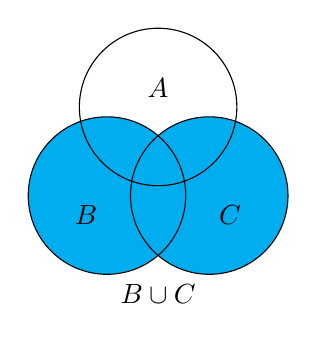
\begin{tikzpicture}
    \fill[cyan] \thirdcircle;
    \fill[cyan] \secondcircle;
    \draw \firstcircle node[text=black,above] {$A$};
    \draw \secondcircle node [text=black,below left] {$B$};
    \draw \thirdcircle node [text=black,below right] {$C$};
    \node[below] at (current bounding box.south) {$B \cup C$};
\end{tikzpicture}
\hfill
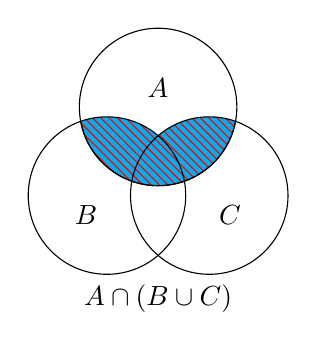
\begin{tikzpicture}
    \begin{scope}
        \clip \firstcircle;
        \fill[cyan] \secondcircle;
        \fill[cyan] \thirdcircle;
    \end{scope}
    \begin{scope}
        \clip \secondcircle \thirdcircle;
        \draw[pattern=north west lines, pattern color=red] \firstcircle;
    \end{scope}
    \draw \firstcircle node[text=black,above] {$A$};
    \draw \secondcircle node [text=black,below left] {$B$};
    \draw \thirdcircle node [text=black,below right] {$C$};
    \node[below] at (current bounding box.south) {$A \cap \left(B \cup C\right)$};
\end{tikzpicture}
\\ \\
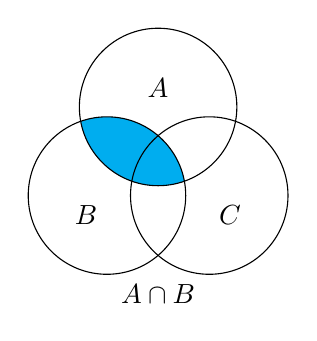
\begin{tikzpicture}
    \begin{scope}
        \clip \firstcircle;
        \fill[cyan] \secondcircle;
    \end{scope}
    \draw \firstcircle node[text=black,above] {$A$};
    \draw \secondcircle node [text=black,below left] {$B$};
    \draw \thirdcircle node [text=black,below right] {$C$};
    \node[below] at (current bounding box.south) {$A \cap B$};
\end{tikzpicture}
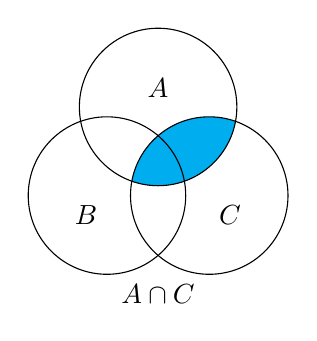
\begin{tikzpicture}
    \begin{scope}
        \clip \firstcircle;
        \fill[cyan] \thirdcircle;
    \end{scope}
    \draw \firstcircle node[text=black,above] {$A$};
    \draw \secondcircle node [text=black,below left] {$B$};
    \draw \thirdcircle node [text=black,below right] {$C$};
    \node[below] at (current bounding box.south) {$A \cap C$};
\end{tikzpicture}
\hfill
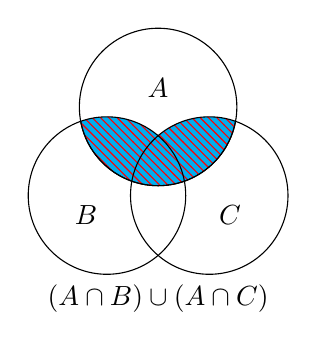
\begin{tikzpicture}
    \begin{scope}
        \clip \firstcircle;
        \fill[cyan] \secondcircle;
        \fill[cyan] \thirdcircle;
    \end{scope}
    \begin{scope}
        \clip \secondcircle \thirdcircle;
        \draw[pattern=north west lines, pattern color=red] \firstcircle;
    \end{scope}
    \draw \firstcircle node[text=black,above] {$A$};
    \draw \secondcircle node [text=black,below left] {$B$};
    \draw \thirdcircle node [text=black,below right] {$C$};
    \node[below] at (current bounding box.south) {$\left(A \cap B\right) \cup \left(A \cap C\right)$};
\end{tikzpicture}
\\ \\
Thus, \[ A \cap \left(B \cup C\right) = \left(A \cap B \right) \cup \left(A \cap C\right) \]
\\ \\ \\
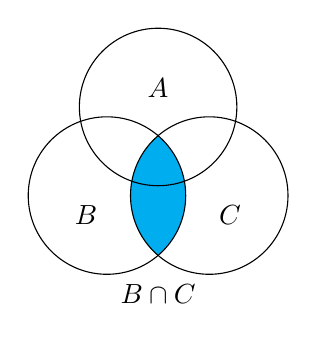
\begin{tikzpicture}
    \begin{scope}
        \clip \secondcircle;
        \fill[cyan] \thirdcircle;
    \end{scope}
    \draw \firstcircle node[text=black,above] {$A$};
    \draw \secondcircle node [text=black,below left] {$B$};
    \draw \thirdcircle node [text=black,below right] {$C$};
    \node[below] at (current bounding box.south) {$B \cap C$};
\end{tikzpicture}
\hfill
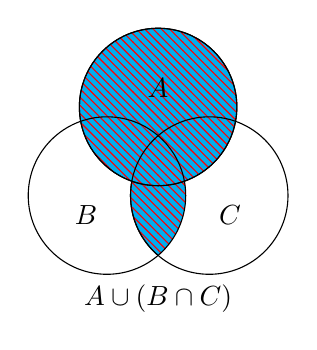
\begin{tikzpicture}
    \begin{scope}
        \clip \secondcircle;
        \fill[cyan] \thirdcircle;
        \draw[pattern=north west lines, pattern color=red] \thirdcircle;
    \end{scope}
    \fill[cyan] \firstcircle;
    \draw[pattern=north west lines, pattern color=red] \firstcircle;
    \draw \firstcircle node[text=black,above] {$A$};
    \draw \secondcircle node [text=black,below left] {$B$};
    \draw \thirdcircle node [text=black,below right] {$C$};
    \node[below] at (current bounding box.south) {$A \cup \left(B \cap C\right)$};
\end{tikzpicture}
\\ \\
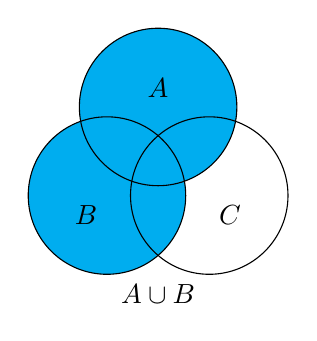
\begin{tikzpicture}
    \fill[cyan] \firstcircle;
    \fill[cyan] \secondcircle;
    \draw \firstcircle node[text=black,above] {$A$};
    \draw \secondcircle node [text=black,below left] {$B$};
    \draw \thirdcircle node [text=black,below right] {$C$};
    \node[below] at (current bounding box.south) {$A \cup B$};
\end{tikzpicture}
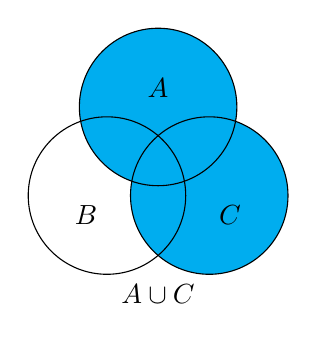
\begin{tikzpicture}
    \fill[cyan] \firstcircle;
    \fill[cyan] \thirdcircle;
    \draw \firstcircle node[text=black,above] {$A$};
    \draw \secondcircle node [text=black,below left] {$B$};
    \draw \thirdcircle node [text=black,below right] {$C$};
    \node[below] at (current bounding box.south) {$A \cup C$};
\end{tikzpicture}
\hfill
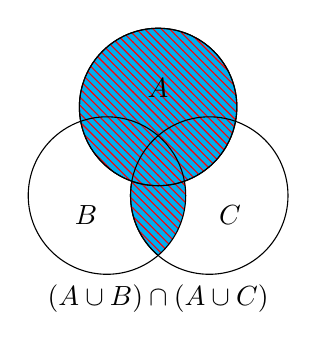
\begin{tikzpicture}
    \begin{scope}
        \clip \secondcircle;
        \fill[cyan] \thirdcircle;
        \draw[pattern=north west lines, pattern color=red] \thirdcircle;
    \end{scope}
    \fill[cyan] \firstcircle;
    \draw[pattern=north west lines, pattern color=red] \firstcircle;
    \draw \firstcircle node[text=black,above] {$A$};
    \draw \secondcircle node [text=black,below left] {$B$};
    \draw \thirdcircle node [text=black,below right] {$C$};
    \node[below] at (current bounding box.south) {$\left(A \cup B\right) \cap \left(A \cup C\right)$};
\end{tikzpicture}
\\ \\
Thus, \[ A \cup \left(B \cap C\right) = \left(A \cup B\right) \cap \left(A \cup C\right) \]


\section*{1.1.3}
\begin{enumerate}[label=(\alph*)]
    \item $f(m) = m^2 + 1$ is a true mapping, but it is neither surjective nor injective:
    \[ f(X) = \{1, 2, 3, \cdots\} \neq \mathbb{Z} \implies \text{Not Surjective} \]
    \[ \forall a \in \mathbb{Z} \quad f(a) = f(-a) \implies \text{Not Injective} \]
    \item $f(n) = n + 1$ is a true mapping and it is injective, but it is not surjective:
    \[ f(X) = \{2, 3, 4, \cdots\} \neq \mathbb{N} \implies \text{Not Surjective} \]
    \item $f(x) = \log x$ is not a true mapping from $\mathbb{Z}$ to $\mathbb{R}$, as $\log x$ is only defined for positive values.
    \item $f(x) = e^x$ is a true mapping and it is injective, but not surjective:
    \[ f(X) = \{x; x\in\mathbb{R}, x>0\} \neq \mathbb{R} \implies \text{Not Surjective} \]
\end{enumerate}


\section*{1.1.4}
\begin{enumerate}[label=(\alph*)]
    \item $f$ is surjective for all tripples $(0, 1, c)$, as any line with slope 1 and integer y-intercept will hit all other integers.
    \item $f$ is injective for all tripples $(0, b, c)$, as any non-zero value for $a$ will result in a `parabola'.
\end{enumerate}



\end{document}